\newcommand{\addr}[1]{\texttt{#1}}

%Visual debugging can be a valuable method to identify and correct
%errors in simulation software.  Current approaches, however,
%are limited by the traditional workflows ascribed to the \emph{use} of
%simulation software. We endeavor to enable \textit{in situ}
%understanding of simulation data.

%The massive size of current and future data is a cause of great concern
%among the visualization community. \textit{In situ} visualization
%provides one of the most promising approaches for dealing with
%the data deluge.  However, the coupling between visualization and
%simulation tool---including the ongoing maintenance such a coupling
%implies---limits the
%application of \textit{in situ} visualization to a small set of
%technically-inclined users.
%
%This coupling is fundamentally rooted in the exchange of metadata that
%describes the data model and data structures of the simulation code to
%the visualization tool.  In this work, we demonstrate that a data model
%and a simulation program are enough information to fully parameterize
%the data structure metadata for \textit{in situ} visualization,
%obviating the need for coupling code and auxiliary descriptions of data
%arrays and information.

Simulation software is routinely used by many disciplines to understand
phenomena when traditional measurement is impractical or even
impossible.  As models increase in detail, however, and the software
stacks underlying high-performance simulation code expand, developing
simulations consequently grows in difficulty.  Verification and
validation of a simulation is therefore an increasingly critical task.
Visualization serves a prominent role in this process, but similar
complexity concerns weigh heavily on the development of new simulation
techniques.

To address the high cost of coupling visualization with simulation
code, we have developed a novel approach that obviates the need for
an explicit connection.  Through instrumented execution of native
x86-64 assembly, we cheaply segment out data of interest and infer the
metadata required for visualization.  As our analysis is binary-level,
it works with any of the languages popular in the high-performance
computing domain.  This transient coupling can be applied or removed
in an \textit{ad hoc} manner.  We demonstrate the utility of the
approach with a number of microbenchmarks and real-world simulations
in use by current researchers.

\definecolor{darkcyan}{rgb}{0.1,0.5,0.6}
\definecolor{darkgreen}{rgb}{0.1,0.6,0.1}
\lstset{
  commentstyle=\color{darkgreen},
  keywordstyle=\color{red},
  identifierstyle=\color{black},
  keywords="size_t",
  frame=none,
  captionpos=b,
  numbers=none,
  numberstyle=\tiny\color{gray},
}

\section{Introduction}

%what/why sim
%vis is necessary
%existing coupling solutions (e.g. VisIt's libsim) are difficult to integrate
%dream: visualization is *concurrent* with simulation development

%data in a simulation program can be considered one of a few (finite)
%  parameterized types
%if we have the parameterized type for a data set, we can create a visualization
%  for it
%most \textit{in situ} tools rely on APIs to transmit this information from
%  simulation to visualization
%the APIs for transmittance are what makes this difficult

%two things make in situ vis hard:
%  * linking in massive software stack for visualization tool
%  * coding to the aforementioned API for communicating data \&\& metadata
%if we could remove these aspects, we're one step closer to the dream.  but how
%do we communicate the metadata without explicit communication?

%simulation does not `do' much, in comparison to most application software
%that is, a simulation spends most of its time in inner loops, repeating the
%  same computation
%this means there isn't too much data that isn't "data of interest": something
%  we might want to visualize
%we can get a small set by automatic means (no strings, etc.)
%when small enough, user interaction can reduce the set to a manageable size
%  \* enzo made 2,028 allocations in a sample run i did.  this is a small \#!

%\todo{histogram of memory lifetimes? can use it to make the point that
%most memory is short-lived}

%\todo{this appears to address Vis people and Sim people, but we're
%publishing it in a PL conference.  Addressing the wrong people, need to
%change focus!}

%\todo{can probably make the point that vis and sim can go together in
%smaller amount of text}

Simulation has seen tremendous growth as a tool to understand problems
from biomedicine to engine design, epidemiology, atmospheric systems,
and many more scientific disciplines. In developing and debugging
such simulations, validation is a difficult yet necessary process.
The inability or cost of performing experimental comparison is often
prohibitive.  Even when measured experimental scenarios exist,
oftentimes comparisons to the measurements are best done in a visual
way.

%% add here that we need to do in situ so that it makes the process feasible

The traditional cycle for simulation-based understanding begins with
editing the simulation's code, running some example systems and dumping
potentially large amounts of data to disk, and finally loading the data
into a visualization tool for analysis.  To accelerate the cycle time
in this `waterfall' process, many simulation authors are turning to
\textit{in situ} visualization: pre-baking the visualization task so
that it can be
produced \emph{while} the simulation is running.  Dynamic control (i.e.
editing of the visualization task at runtime) is possible, but has
remained elusive in practice.

The nature of these as discrete steps is unfortunate.  A simulation
author might not consider visualization until the simulation
itself is fully written.  Yet the ability to \emph{see} the effect of
code modifications on the simulated data could have a profound effect
on the productivity of the simulation author.  We believe part of what
holds back dynamic visualization of simulation data is the difficulty
in integrating visualization tools into simulation development.

% need to find a way to say this that's not offensive to comp.al scientists
These difficulties are twofold.  The first issue is that visualization
software is often orders of magnitude more complex than simulation
software, and the former requires an extensive set of middleware for
its underlying software stack.  The second is common to using any
library: the simulation author must learn the API and data model that
the visualization tool uses to communicate data and metadata.

\cite{Hall:2009:Next50}~note the importance of ``program-analysis strategies to
improve software construction, maintenance, and evolution.''  In this
work, we introduce a methodology for ``0 day'' coupling of simulation
and visualization code.  We remove the need to link in any external
code to the simulation.  The simulation software does not even need to
be recompiled.  The bulk of our contribution is in the form of program
understanding: we demonstrate how to infer which data
are interesting \emph{as well as}---more importantly---the
parameterization of those data that enables visualization.  This
obviates the need for the simulation author to conform to, or even
learn, an external API.

%Some simulation authors are turning to \textit{in situ} techniques for
%effective high-performance visualization, especially as simulations
%begin dumping more data than can be processed via a traditional
%`staged' pipeline.  These techniques consider the complete process of
%understanding phenomena, with simulation and visualization as a single
%intertwined symbiotic stage.  This fuels large efficiency increases, at
%the cost of a measure of flexibility.

%The small scale of the visualization community in relation to the
%simulation community's size has imposed a particular and often
%ill-acknowledged collaborative structure.  Notably, the visualization
%community must produce tools that the simulation community consumes.
%In the case of \textit{in situ} visualization, the visualization
%community produces \textit{in situ} tools, and individual simulation
%authors are tasked with coupling those visualization tools with their
%simulation.
%
%We feel that this merger between simulation and visualization tool
%imposes a significant tax on the simulation author.  Furthermore,
%background dynamics of both communities disenfranchise the simulation
%author to effect this symbiosis: commonly, simulation authors are
%domain experts, and visualization experts come from a computer science
%background.  Frequently, visualization community members have formal
%and practical training in the construction of software, whereas a
%simulation author who is both a domain expert \emph{as well as} an
%experienced software developer is cherished for their abilities.
%
%As an alternative to the status quo in the communities' interaction,
%visual validation, and the traditional \emph{in situ} visualization
%approaches, we propose a novel system that automatically identifies and
%interprets visualizable fields in a running simulation.  No special
%effort is required on the part of the simulation author.  Visualizable
%data is presented concurrently with simulation results and updated
%automatically as the simulation evolves.  The ease of use encourages
%simulation authors to include visual debugging in their regular
%development cycle, much in the way a read-eval-print-loop (REPL)
%encourages users to experiment and evaluate language constructs.

\section{Program analysis and assumptions}
\label{sec:model}

In this section we develop an abstract model of an executing simulation
program.  Our model utilizes a machine that is a significant
simplification from our target architecture of x86-64, but our analysis
only requires this high-level specification.

%While the model is restrictive, architectural realities, the state
%of modern compiler capabilities, and modern software development
%`best practices' make the simplifications largely irrelevant for our
%purposes.  We then use the model to infer data of interest.

\begin{lstlisting}[float=*,label=lst:relaxation,language=C,caption=A code
fragment representative of simulation software.  A large array is smoothed using
a set of nested loops. \texttt{S} is presumed to be a macro that
samples \texttt{data} while properly accounting for edge cases.]
for(size_t j=0; j < dims[1]; ++j) {
  const size_t row = j*dims[0];
  for(size_t i=0; i < dims[0]; ++i) {
    data[row+i] = (S(x-1,y-1) + S(x-0,y-1) + S(x+1,y-1) +
                   S(x-1,y-0) + S(x-0,y-0) + S(x+1,y-0) +
                   S(x-1,y+1) + S(x-0,y+1) + S(x+1,y+1)) / 9.0
  }
}
\end{lstlisting}

The code fragment in Listing~\ref{lst:relaxation} fits the model of the
software of interest to us in this work.  Assuming such code is found
in an environment that greatly emphasizes high-performance implies much
about the code displayed here.  First, the
\texttt{data} array can only be a multidimensional array (even though
its type is one-dimensional).  That array must be heap-allocated using
a single allocation request: simulations routinely deal with data
sizes far larger than typical stack or static memory sizes.  Data flow
analysis would identify
the access of \texttt{data} within the loops of
Listing~\ref{lst:relaxation} as dependent on the loop variables
\texttt{i} and \texttt{j}, though there is little need for such
formality: both the programmer and the compiler would have strong
incentives to hoist the access, were this not the case.  Finally,
\texttt{data}'s dimensionality in this program must be two, and the
number of elements is $dims[0] \times dims[1]$.

\newcommand{\pointsto}[0]{\rightarrow}
\newcommand{\union}[0]{\cup}

\begin{figure}
\begin{eqnarray}
  BaseType &:=& Booleans \union Integers \union FP
    \union Strings \nonumber\\
  Type &:=& BaseType \union Array \union Pointer \nonumber \\
  Memory &:=& Heap \union Static \union Local
    \union Arguments \union Text \nonumber \\
  IPtr &\in& Text \nonumber\\
  T &:=& Memory \mapsto Type \nonumber \\
  B &:=& Memory \mapsto BaseType \nonumber \\
  F &:=& [ addr \in Text, end \in Text ]  \mid \  addr < end \nonumber\\
  W &:=& Text \mapsto F \nonumber \\
  %\textbf{class} & \  Node_{CFG} & \  address \  edges \nonumber\\
  \textbf{class} && \  Node_{CFG} \  address \  edges \nonumber\\
  % we have a hole here: need to say a CFG is a set of Node_{CFG}s.
  \indent CFG &:=& \{ n \mid n = Node_{CFG} \} \nonumber\\
  % note that this definition disallows self-modifying code.  that's OK.
  Wr &:=& (m \in Text) \mapsto (n \in (Memory \setminus Text)) \mid m \neq n
    \nonumber\\
  Rd &:=& (m \in Text) \mapsto (n \in (Memory \setminus Text)) \mid m \neq n
    \nonumber\\
  % we have a hole here: need to say a CFG is a set of Node_{CFG}s.
  BB &:=& F \mapsto CFG \nonumber \\
  K &:=& Text \mapsto Node_{CFG} \nonumber\\
  H &:=& Node_{CFG} \mapsto Boolean \nonumber\\
  L &:=& Node_{CFG} \mapsto Integer \nonumber
 %Q := Text \mapsto F\\
%  \textbf{class} \  ND \  base \  length \  dims \  ndims\\
%  \indent | base \pointsto m \in Heap\\
%  \indent | B(base) \in FP\\
%  \indent | T(dims) \in Array \union Pointer\\
%  \indent | B(dims) \in Integer\\
%  \indent | T(ndims) \in Integer\\
%  \indent | ndims > 0\\
%  \indent | Wr(IPtr) \in [ base, base + length ]\\
%  \indent | b \in BB(W(IPtr)) \land IPtr \notin b \land H(b)
%    \land L(K(IPtr)) > L(b)\\
\end{eqnarray}
  \caption{Definitions for abstract machine and analysis based on
  properties of control flow.}
  \label{fig:model}
\end{figure}

We use the formalisms given in Figure~\ref{fig:model}.  We consider an
abstract machine described by an
\textit{instruction pointer} and the current state of
\textit{memory}.
%\begin{math}
%  \indent IPtr \in Text\\
%  \indent Memory := Heap \union Static \union Local \union Argument
%    \union Text\\
%\end{math}
The instruction pointer is assumed to advance automatically, and memory
operations consist of reads and writes that map an address to a mutable memory
location.
%\begin{math}
%  \indent Wr = m \in Text \mapsto n \in (Memory \setminus Text) \mid m \neq n\\
%  \indent Rd = m \in Text \mapsto n \in (Memory \setminus Text) \mid m \neq n\\
%\end{math}
Note that this definition denies self-modifying code.  Memory is assumed to be
\emph{typed}, with a small set of available types.  The $T$ and $B$ mappings
define mappings from memory locations to type information.
%\begin{math}
%  \indent BaseType = Booleans \union FP \union Integers \union Strings\\
%  \indent Type = BaseType \union Array \union Pointer\\
%\end{math}
%and mappings from memory locations to type information.
%\begin{math}
%  \indent T = Memory \mapsto Type\\
%  \indent B = Memory \mapsto BaseType\\
%\end{math}

The running process is assumed to consist of a series of
\textit{functions}, $F$, that are defined as the functions' upper and
lower addresses.  We will make use of an inverse mapping $W$ that
allows us to identify a function from the
current instruction pointer.
%\begin{math}
%  \indent F = [ addr \in Text, end \in Text ] \mid addr < end\\
%  \indent W = Text \mapsto F\\
%\end{math}
We build local \textit{control flow graph}s (CFGs) that describe the potential
execution paths.  These graphs are represented as a set of \textit{nodes} that
contain an entry \textit{address} as well as a set of \textit{edges}.
%\begin{math}
%  \indent \textbf{class} \  Node_{CFG} \  address \  edges\\
%  % we have a hole here: need to say a CFG is a set of Node_{CFG}s.
%  \indent CFG = \{ n \mid n = Node_{CFG} \}\\
%\end{math}
We build these CFGs based on the
function address range.  We define a mapping $K$ that allows
us to identify nodes in the control flow graph from an instruction
address.
%\begin{math}
%  \indent BB = F \mapsto CFG\\
%  \indent K = Text \mapsto Node_{CFG}\\
%\end{math}
We define two final mappings from a node in the control flow graph: 1)
a predicate identifying \textit{loop headers}, and 2) a mapping for the
calculated \textit{loop depth}.  The headers $H$ correspond to the
basic blocks that contain the loop test.  In Listing~\ref{lst:relaxation},
the basic blocks containing \texttt{j < dims[1]} and \texttt{i <
dims[0]} would be the loop headers.  Loop depth is the nesting level of
the provided basic block.  In Listing~\ref{lst:relaxation}, the
assignment to \texttt{row} has a depth of $1$.  The assignment to the
element in \texttt{data} has a loop depth of $2$.
%\begin{math}
%  \indent H = Node_{CFG} \mapsto Boolean\\
%  \indent L = Node_{CFG} \mapsto Integer\\
%\end{math}

%\noindent \begin{math}
%  BaseType := Booleans \union Integers \union FP \union Strings\\
%  Type := BaseType \union Array \union Pointer\\
%  Memory := Heap \union Static \union Local \union Arguments \union Text\\
%  IPtr \in Text\\
%  T = Memory \mapsto Type\\
%  B = Memory \mapsto BaseType\\
%  F := [ addr \in Memory, end \in Memory ] | addr < end\\
%  W := Text \mapsto F\\
%  % note that this definition disallows self-modifying code.  that's OK.
%  Wr := (m \in Memory) \mapsto (n \in Memory) | m \neq n\\
%  \textbf{class} \  Node_{CFG} \  address \  edges\\
%  % we have a hole here: need to say a CFG is a set of Node_{CFG}s.
%  BB := F \mapsto CFG\\
%  K := Text \mapsto Node_{CFG}\\
%  H := Node_{CFG} \mapsto Boolean\\
%  L := Node_{CFG} \mapsto Integer\\
%  %Q := Text \mapsto F\\
%  \textbf{class} \  ND \  base \  length \  dims \  ndims\\
%  \indent | base \pointsto m \in Heap\\
%  \indent | B(base) \in FP\\
%  \indent | T(dims) \in Array \union Pointer\\
%  \indent | B(dims) \in Integer\\
%  \indent | T(ndims) \in Integer\\
%  \indent | ndims > 0\\
%  \indent | Wr(IPtr) \in [ base, base + length ]\\
%  \indent | b \in BB(W(IPtr)) \land IPtr \notin b \land H(b)
%    \land L(K(IPtr)) > L(b)\\
%\end{math}

Using this model of program execution, we consider the problem of
automatically identifying memory regions that house data that a user
would want to visualize.  We model these as a set of constraints on
type classes.  An instance of the type class allows one to visualize
data within a simulation.

%, with constraints sourced from the observation of program
%execution.  In this way, we can visualize the data \emph{as} it is
%modified by the simulation.

%\todo{haven't actually convinced myself this is a type class in the
%correct sense of the term, based on my limited understanding of it.
%maybe `constrained parametric type' is better. it certainly resonates
%better with me...}

The type we search for is the $N$-dimensional (``ND'') data array.
This type is parameterized by a \texttt{base} address, a
\texttt{length} (in bytes), the number of
dimensions \texttt{ndims}, an array of dimensions \texttt{dims}, and
finally the type of the data.
% need a 'comment' column to summarize important considerations!
\begin{eqnarray}
  \indent \textbf{class} \ & ND & \  base \  length \  ndims \  dims \  type
    \nonumber\\
  \indent &\land& base \pointsto m \in Heap\\
  \indent &\land& B(base) = type\\
  \indent &\land& T(dims) \in Array \union Pointer\\
  \indent &\land& B(dims) \in Integer\\
  \indent &\land& T(ndims) \in Integer\\
  \indent &\land& ndims > 0\\
  \indent &\land& Wr(IPtr) \in [ base, base + length ]\\
  \indent &\land& \exists b \in BB(W(IPtr)) : \nonumber\\
    && \land \ IPtr \notin b \nonumber \\
    && \land \ H(b) \nonumber\\
    && \land \ L(K(IPtr)) > L(b)
\end{eqnarray}
We use the $\pointsto$ notation to mean ``points to''; the first
constraint simply states that the data of interest live on the heap.
As simulation data is large, it cannot fit on the stack or even in
statically initialized memory.  The second constraint conveys that the base
type matches a parameter of our model, such as $FP$ (floating point).
The third and fourth constraints dictate that the dimensions are stored
in a linear list of integers, and the fifth and sixth say the variable
that describes the length of that list is a simple integer.

The 7th and 8th constraints are complex and intertwined.  First, the
application must write into the the relevant memory block.  Secondly,
the basic block where the data are written must be deeper than another
basic block that contains a loop header.  That is to say that the data
access occurs within a loop.

The formulation gives rise to a pattern matching problem.  The
\texttt{\textbf{class}}es of interest are the patterns, and the space
to match within is the running process' \texttt{Memory} and
\texttt{IPtr}.  In Listing~\ref{lst:relaxation}, the parameter bindings are:
\texttt{data} for \texttt{base}, the size of the allocation (not shown, but
assumed to be \texttt{dims[0]} $\times$ \texttt{dims[1]} $\times$
\texttt{sizeof(float)}) for
\texttt{length}, \texttt{dims} for \texttt{dims}, and $2$ for
\texttt{ndims}.

\section{Implementation}

Our task is to match the given constraints with an executing process.
Working with the executing process is imperative given our goal of
concurrently visualizing the data as it is computed.  Furthermore, some
constraints---notably those involving the value of variables, such as
the instruction pointer or a variable to be matched such as $ND$'s
(``$N$-Dimensional'')
\texttt{ndims}---can only be determined at runtime.  Therefore the
system must include some level of dynamic analysis.  For simplicity and
applicability, we do all of our analysis during runtime and directly on
the binary under execution.

We target unstripped binaries with debug information.  This gives us
robust type information as well as simplifying implementation.
Reps et al. give detailed information in~\cite{Reps:2010:Bottom} on
how this simplifies the task. Our use case of simulation developers
creating and debugging their simulation coincides with this input: the
environment would make it likely that users would compile with debug
information even without our tool in use.

A notable advantage of targeting binaries is that it is
language-agnostic.  C, C++, and Fortran are the dominant programming
languages used in high-performance computing environments.  By parsing
machine code for our target x86-64 platform we simplify the entire
system by dealing ostensibly with a single input language.  %A %set of
%reasonable assumptions for the executing process and environment %is
%given in
%\S{\ref{sec:assumptions}}.
Given these assumptions and the simplifications of our model in
Section~\ref{sec:model}, the transformation from a language such
as C to assembly language preserves all information of relevance.

Our system uses a \texttt{ptrace(2)}-based supervisor for the target
program.  We induce small changes to process execution that are
invisible under memory-safe operation, and our efforts are rewarded
through efficient notification of events in the simulation.  An example
event is the access of a data array previously identified as housing
visualizable data.
When such events are \emph{not} occurring, simulation execution
proceeds at native speed.

% governed by a finite state machine (see fig 1)
% every memory (allocation) region is at some state in state machine
% we don't actually need to instantiate a state machine for each allocation
%% those in the 'null' state can be ignored

Heap-allocated memory is the centerpiece of each
\texttt{\textbf{class}} we search for.  Any heap-allocated memory
region is potentially of interest for us, though we note that at any
given moment, most allocations provide uninteresting input from a
visualization standpoint. We model each memory region by the finite
state machine given in
Figure~\ref{fig:fsm}, with the initial `null' state represented
implicitly for efficiency reasons.  All memory is assumed to be in the
`null' state initially.  Memory regions change their state based on
events observed in the simulation process.  Note that a single event
may cause a transition in multiple regions.

\begin{figure}
  \centering
  \begin{tikzpicture}[scale=1.0,thick,align=center]
    \node[state](null){null};
    \node[state,right of=null](mloc){malloc};
    \node[state,above of=mloc](mret){mreturn};
    \node[state,right of=mret](allow){allow};
    \node[state,below of=allow](kill){kill};
    \node[state,below of=kill](deny){deny};
    \node[state,left of=deny](hdr){header};
    \path[line](null)--(mloc);
    \path[line](mloc)--(mret);
    \path[line](mret)--(kill);
    \path[line](mret)--(allow);
    \path[line](allow)--(kill);
    \path[line](allow)--(hdr);
    \path[line](allow) to[out=-20,in=0] (deny);
    \path[line](hdr)--(kill);
    \path[line](hdr)--(deny);
    \path[line](hdr) to[out=180,in=120,distance=1cm] (hdr);
    \path[line](deny) to[out=20,in=0] (allow);
    \path[line](deny)--(kill);
    \path[line](kill) to[out=-200, in=60] (null);
  \end{tikzpicture}

  \caption{Finite state machine governing memory regions of interest.
  Regions transition between the states based on events observed in
  the observed simulation process.  Basic information is obtained in
  the \emph{malloc} and \emph{mreturn} states.  The \emph{allow} state
  initializes parameters for visualization and enables unfettered
  access to the memory. \emph{header} states build up the dimensions of
  the data.  The \emph{deny} state is used to detect future accesses.
  Memory is \emph{kill}ed when it is deallocated.}
  \label{fig:fsm}

\end{figure}

\subsection{Memory tracking}

The events that instantiate the memory regions of interest are
allocation requests.  We implement the event notification by
inserting a breakpoint on \texttt{malloc} calls, and can thereby track
all heap memory in use by an application.  When the breakpoint is hit,
we examine the argument to determine the size of the allocation.  A
second breakpoint is inserted when
\texttt{malloc} returns, to read the pointer the call produced.
Together, these allow us to identify the base addresses and lengths
of all the heap memory in the process.  Overhead for this aspect is
predominantly context switching from the simulation process to the
supervisor.

The $ND$ \texttt{\textbf{class}} has constraints that include the
function pointer at the time the data (memory within \texttt{base} and
\texttt{base} $+$ \texttt{length}) were accessed.  Unfortunately, the
\texttt{malloc}-based tracking only informs us what dynamic memory
\emph{exists} in a process, not when it is \emph{accessed}.
Traditional debugger watchpoints are implemented (on x86*
architectures) using a finite set of debug registers; these would be
quickly exhausted in our case.  Finding instructions that modify memory
and inserting checks is a viable
alternative, but~\cite{Antoniu:2001:PFault} previously showed this to
be inefficient.

%Tracking the pointer via symbolic interpretation may be possible, but
%quickly runs up against difficult-to-solve aliasing problems, and is
%unlikely to be computationally viable.

We use a technique from distributed shared memory environments that
induces a segmentation fault when the data of interest are accessed.
We subtly alter every allocation of interest so that it not only
allocates the memory, but also protects the memory region, as per the code
shown in Listing~\ref{lst:malloc}.  When the process attempts to alter
the data of interest, the memory
protection hardware traps and our supervisor is notified\footnote{The
program may also trap because it has a bug that causes an invalid
memory access.  Such programs are beyond the scope of this work.
Still, we note that we can discern the invalid memory access case and
notify users of the error's location.}

%\begin{minipage}{\linewidth}
\begin{lstlisting}[label=lst:malloc,language=C,caption=Replacement \texttt{malloc}
implementation used for tracking field access.]
void* alignedalloc(size_t n) {
  void* mem;
  if(posix_memalign(&mem, getpagesize(), n) != 0) {
    return NULL;
  }
  if(mprotect(mem, n, PROT_READ) != 0) {
    free(mem);
    return NULL;
  }
  return mem;
}
\end{lstlisting}
%\end{minipage}

As this segmentation handling is expensive, we only perform access
detection for the first access within a function.  After it detects a
segmentation fault in the simulation process, our supervisor changes
the memory protections to allow unfettered access to the data.  At
the same time, we insert a breakpoint at the caller of the current
function, so that we may re-enable memory protection and detect
subsequent accesses of the same data.

The astute reader may note that memory protection is possible only on
page-aligned data.  We therefore require a modified \texttt{malloc}
implementation that calls \texttt{posix\_memalign} (to allocate the
page-aligned memory) followed by \texttt{mprotect} (to set up the
desired memory protections).  Since we do not require the user to link
against any runtime, adding a function in the traditional way is not
viable.  Instead, we inject our modified \texttt{malloc} implementation
directly into the executing process image after static initialization
has completed.  We modify the instruction pointer when a
\texttt{malloc} occurs to instead jump to our page protection
allocation routine.

\subsection{Control flow}

The memory tracking described above enables our supervisor to track
most of the events it needs.  To pinpoint the remaining events we use
analysis based on the local control flow.  When a region is accessed,
we build the local control flow graph for the currently-executing
function.  Our supervisor computes common compiler analysis
information such as dominance~\cite{Torczon:2007:Compiler} and uses
the results of this analysis to define per-node depth as well as to
identify
loop headers, as in Figure~\ref{fig:cfg}.

There are some known limitations to this approach.  One is its
fragility in the presence of
\texttt{goto} statements.  If the \texttt{goto} crosses a loop
boundary, then the depth information calculated may be incorrect, and
the algorithm will not compute a proper loop tree.  Fortunately, in
practice this is rare; we have not encountered this case in simulation
programs of interest.

%% drop this?  it sounds really negative.
Some compiler optimizations pose issues as well.  Loop transformations,
such as loop tiling or fission, can cause issues with the inference we
perform.  While it may be possible to workaround these on a case by
case basis, we reiterate that our use case is primarily in the domain
of simulation \emph{development}.  As such, these optimizations can
simply be disabled during development to allow use of the tool.

%% relies on assumptions:
%%%% data are within the loop because the loop is relevant
%%%% => loop bounds imply bounds on the data
%%%% the application does not use gotos in these tight loops
%%%% loop tiling etc. are not performed
\begin{figure}
  \centering
  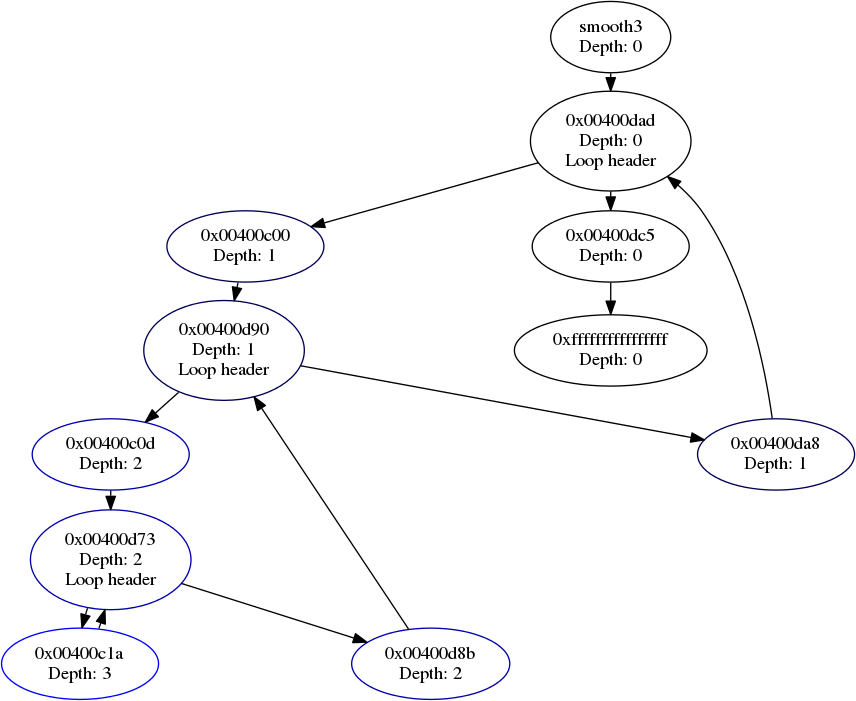
\includegraphics[width=\linewidth]{images/dbg/s3}

  \caption{Simplified control flow graph for a small function that
  smooths a 3D array.  Analysis identifies loop headers and the nesting
  level (`Depth') of each basic block.  On access, the loop tree is
  traversed to determine the dimensionality of the array.}

  \label{fig:cfg}
\end{figure}

\subsection{Symbolic execution}

As described in the $\textbf{class} \ ND$ of Section~\ref{sec:model},
we assume a relation between loop headers and the basic blocks that are
contained within those loops and accessing memory.  The loop variable
must be involved: if it were not, the access would be loop-invariant
and hoisted out of the loop, either explicitly by the programmer or
implicitly by the compiler.  We assume a stronger relation, however:
that the loop conditions imply the dimensionality of the memory regions
accessed therein.

%\todo{this is very strong, which is okay, but we have no proof, which
%is not okay} Barring absurd instruction sequences (e.g. a series of
%\texttt{NOP}s), there are a finite number of ways that a compiler might
%encode a loop header.

Since the loop header decides whether the loop will continue or not, it
must reference both the induction variable and the loop bound.  If we
can identify which operand is which, then we will know the loop bound.

The comparison instruction itself has no ordering or other method to
distinguish the operands.  We utilize the debug information to decide
whether each operand is a local, reference to a global, or a constant.
When exactly one of these references is a local, we consider it the
induction variable; the other variable gives the loop's bound.

\begin{lstlisting}[label=lst:header,caption=Instructions within a
sample loop header.  Both the induction variable and the loop bound
appear as arguments to the \texttt{CMP} instruction.  The preceding
instructions are still necessary for distinguishing between the two
variables.]
  MOV %rdx, [%rip+0x20507]
  MOV %rax, [%rpb-0x60]
  CMP %rdx, %rax
  JB -0x275
\end{lstlisting}

%% bad: 'we'd like to do X, but it's too impossible, so we do Y.'
Ideally, we would simply examine the comparison instruction to identify
the operands and infer the loop bound. Unfortunately a myopic view of
this single instruction is insufficient for operand classification.
The instruction sequence for a loop header generally follows the
pattern that
Listing~\ref{lst:header} follows: first, the bound and induction
variables are loaded into registers; second, the comparison is
performed; and finally, a conditional jump exits the basic block.  The
induction and bound variables are referenced in the basic block, but
the comparison itself often operates on registers that have erased the
original source of the data.  Concretely, in Listing~\ref{lst:header},
\texttt{\%rax} itself is less relevant than the \emph{source} of
\texttt{\%rax}'s
value: the memory pointed to by \texttt{\%rbp-0x60}.  Since the variable
is relative to the frame pointer, this tells us that it must be an
argument or a local variable.  Debug information for the program can
discriminate between these final two cases for us.

% the LH basic block must reference both the induction variable as well as the
%   end criterion
%%%% we could prove this empirically.  just take enzo, for example, compute the
%%%%  CFG for every function, and then analyze each loop header to check if it
%%%%  loads two things.
% "myopic view of CMP" is not enough
%% no ordering to the operands! how do we identify what kind of thing we have?
%%% the induction variable can be safely assumed to be a local
%%% the end criterion *might* be local, but more likely a constant, argument
%%%   to the current function, or a global.
%%%%% again, we could empirically verify: is every CMP in an enzo LH a
%%%%% combination of a local and a (constant | argument | global)?
%% we can solve the type information problem using debug information
%%% but again: myopic view of CMP is not enough

\begin{algorithm}
  \caption{Symbolic interpretation algorithm for identifying data sources.  A
  virtual register set is tracked within loop-free basic blocks to identify
  the source of operands to specific instructions.  These sources are then
  used to lookup debug information and interpret register contents.}
  \label{alg:sinterp}
  \begin{algorithmic}[1]
    \State register[*] := UNKNOWN
    \State instruction := bb$_{addr}$ \Comment first instruction in loop header
    \Repeat \Comment foreach instruction in the basic block
      %\Comment cast to instruction of appropriate type
      \State \Comment cast to instruction of appropriate type
      \If{instruction.Opcode = MOVE}
        \State mov := (MovInstruction)instruction
        \If{mov.source $\in$ register}
          \State register[mov.target] := register[mov.source]
        \ElsIf{mov.source is an address}
          \State register[mov.target] := mov.source + \\
                                         \hspace{6em}memdiff[mov.source]
        \EndIf
      \EndIf
      \State \Comment Track address modifications
      \If{instruction.Opcode = ADD}
        \State add := (AddInstruction)instruction
        \If{add.dest $\in$ register $\land$ \\
            \hspace{3.75em} register[add.dest] $\neq$ UNKNOWN}
          \State register[add.dest] += add.source
        \EndIf
        \If{add.dest $\in$ memory}
          \State memdiff[add.dest] += add.source
        \EndIf
      \EndIf
      \State instruction := next(instruction)
    \Until instruction.Opcode = CMP
  \end{algorithmic}
\end{algorithm}

Algorithm~\ref{alg:sinterp} derives the source of the data in the loop
header's comparison instruction.  We track a virtual register set
and the set of memory changes over the basic block of the header's
instruction sequence.  Instructions that modify a register or memory
are tracked, though only the differences to memory operations are
saved.  The interpretation terminates at the basic block's comparison
instruction, and outputs the symbolic register file.  We can use this
register file to identify the source of the data within a comparison
instruction.

%% again, a negative and really minor case.  can't we just drop this?
It can occur that the loop bound is also a local variable, making
both the induction variable and the bound both local.  This impedes
our ability to discern the bound operand.  However, we note that this
situation is unlikely to occur in practice.  If the dimensionality of
the array does not change during execution of the function, then this
local variable for the bound should also not change: in this case,
the compiler is likely to elide the variable in favor of a constant.
Our fallback case is to choose the larger of the two values in the
comparison, however we note that we have not yet hit this case in
simulation code utilized thus far.

Once we have identified the source of the data in the comparison
instruction, we allow the simulation to run to that point.  We use
\texttt{ptrace(2)} to read the value for the loop bound.  To interpret
the value, the virtual register set gives the key for the debug
information needed.

%Integer-based or pointer-based indices is at present an input to our
%model that the user must specify, with ill-developed semantics for
%the pointer case.  In the future, we hope to detect this case using
%debug information to automatically choose between the two.  Pointer
%comparisons as opposed to integer indices may pose issues due to the
%ambiguous mapping from the addresses to indices accessed.  For the
%future, we plan to assume a linear traversal of the data and compute
%the indices based on the allocation's type as well as the starting and
%ending indices.  In practice, this case happens so rarely in simulation
%code that we simply ignore loops of this type.

Each iteration of this process gives a single loop bound.  By following
the
state machine in Figure~\ref{fig:fsm} and setting breakpoints up the
chain of the loop tree, we derive the full set of bounds.  At the
function boundary, we enter the `deny' state and re-enable memory
protection for that region.

\section{Evaluation}

%\todo{be more excited about how great this is}
%
%\todo{constantly mentioning the drawbacks and "the 1\%" cases that
%fail, but they're not a big deal---mention those later}

% our stuff is the greatest thing since sliced bread

% already found an indexing error in an image smoothing application
%% image: an image side-by-side with a smoothing error that skews in X

% get a figure of a (pretty!) volume rendering in here

\textit{In situ} visualization is commonly applied in large-scale
parallel simulations in order to reduce the cycle time from simulation
setup to data understanding.  The approach is primarily motivated by
performance: visualization that runs concurrently with the simulation
does not need the costly data loading step common at the start of most
visualization pipelines.  Our thesis is orthogonal to this original
purpose: that \textit{in situ} visualization is useful during
\emph{development} to visually verify the calculations performed
therein.

%\begin{figure}
%  \centering
%  % \includegraphics ...
%
%  \caption{Original image (left) and image smoothed by an incorrect
%  smoothing algorithm (right) that skews the image in X.  The indexing
%  error is readily apparent from the preview visualization provided.}
%
%  \label{fig:smootherr}
%\end{figure}

%Figure~\ref{fig:smootherr} details an error uncovered in an image
%processing routine in some software the authors' lab was concurrently
%developing.  There was an indexing error relative to one of the loops'
%induction variables, causing the issue on the right.  Viewing the
%result of the algorithm immediately exposes the error.

We are integrating more advanced visualization techniques into the
software at present.  Figure~\ref{fig:volren} shows a volume rendering
for the volume of tissue activated in a biomedical simulation.  The
image was generated using the
ImageVis3D~\cite{Fogal:2010:Tuvok} desktop volume rendering package.
The connection of our instrumentation suite and this visualization tool
presently relies on serialization to and from files due to limitations
of ImageVis3D, but we hope to rely on in-memory transfers in the near
future.

\begin{figure}
  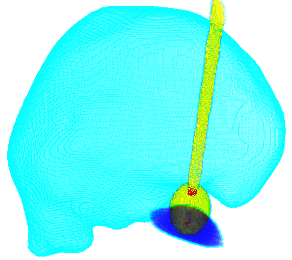
\includegraphics[width=\linewidth]{images/dbg/brain}

  \caption{Volume rendering of the volume of tissue activated from
  a biomedical simulation of deep brain stimulation.  Array shape
  information and data were read from the running simulation and
  serialized to disk, while a concurrent process made the data suitable
  for import into a volume rendering tool.  No user intervention was
  required, beyond setting the transfer function to derive the color
  information.}

%  \caption{Volume rendering of the temperature field from a
%  \textit{PsiPhi} simulation.  Array shape information and data were
%  read from the running simulation and serialized to disk, while a
%  concurrent process made the data suitable for import into a volume
%  rendering tool.  No user intervention was required, beyond setting
%  the transfer function to derive the color information.}

  \label{fig:volren}
\end{figure}

\subsection{Performance}
\label{sec:performance}

A high performance tool encourages simulation authors to integrate that
tool into their daily development routines.  Few developers integrate
useful tools such as Valgrind into their rapid edit-compile-test
cycles, in part due to performance. This functionality is instead
relegated to pre-commit or even nightly testing, limiting the
effectiveness of some memory debugging tools.  Our goal is to enable
visualization that is not only easy to set up, but also cheap enough
that developers leave the tool enabled during daily development.

%\begin{figure}
%  % \includegraphics....
%  %% bar graph of performance w/ and w/o our instrumentation
%
%  \caption{Our `MallocTrace' tool watches for and reports allocation
%  and deallocation requests, producing a report that would be useful in
%  identifying the most promising locations to reduce the application's
%  memory footprint.  It uses breakpoints heavily but no memory access
%  protection; the relatively low overhead indicates that program
%  interruption and interrogation is lightweight.  Software that
%  performs many allocations may experience higher overheads.}
%  \label{fig:mtrace}
%\end{figure}

We therefore consider multiple aspects of performance.  We induce an
overhead in the simulations that we execute by interrupting them at
key points, as well as by minor adjustments to program execution.  The
performance of our supervisor itself is also of interest, as it must
manipulate large symbol tables, construct control flow graphs from
instruction streams, and interpret some instructions to uncover loop
indices.

The approach is evaluated with a set of relevant test programs.
\textit{Linpack} is the matrix-vector multiplication benchmark of
floating point performance that is used to rank supercomputers in the
popular `Top500' list. \textit{Relax} is a program that identifies
the steady state for the case of a plane connected to a constant heat
source.  The program's ratio between function calls and accessing the
data to be visualized is at parity, stressing the memory access and
analysis aspects of our supervisor. \textit{PsiPhi} is a real-world
computational fluid dynamics solver that focuses on Large Eddy
Simulation (LES) of flows that include combustion and other types of
chemical reactions~\cite{Proch:2014:PsiPhi}. \textit{allocs} is a test
program that simply allocs and frees memory without ever acessing it.

Figure~\ref{fig:performance} looks at multiple aspects of performance
across this set of programs.  The red `Uninstrumented' bar details the
execution time without our instrumentation applied, representing an
upper bound for performance.  `Trace' inserts breakpoints at
`\texttt{malloc}', `\texttt{free}', and their return addresses,
measuring what it costs to start and stop the execution of the
simulation program.  Simulations which utilize more regions of dynamic
memory will see higher overheads due to this aspect.  However, the
graph does not capture the phased nature of these processes: generally,
they include a startup phase that allocates memory and initializes
inputs, followed by a computational phase that computes.  As simulation
sizes increase, the initialization phase holds constant whilst the
compute phase scales polynomially.

`Allocations' is a more expensive variant of the `Trace' benchmark.
In addition to allocation interception, this version reads relevant
information from the client process so that it may generate a report
of the [de]allocations made by the process.  The traces this algorithm
creates might be useful in producing and analyzing heap usage over
time, in the same manner as Valgrind's
`Massif'~\cite{Nethercote:2006:Massif}.  We note that this adds little
additional overhead to the instrumentation, demonstrating that reading
memory from the process is cheap.

%As demonstrated by Figure~\ref{fig:mtrace}, the overhead for program
%interruption tied to allocation tracking is low.  All programs profiled
%follow the model of allocating the required memory up front and keeping
%it active for the lifetime of the process.  Thus, most overhead for
%allocation tracking is in a one-time startup phase.  During the
%processes' compute phases, allocations tend to come from external
%libraries, such as the HDF5 file I/O middleware.

`Full' in
Figure~\ref{fig:performance} details overheads for the full gamut of
our analysis techniques.  Conflating the results, however, are filters
that can be applied when more analysis is performed.  As one example of
these
filters, `Full' identifies the caller of \texttt{malloc} and ignores
the allocation if the
memory is an internal \textit{glibc} buffer.  With the extra
information gained from this additional work, `Full' can in many
cases realize that an allocation region is not interesting.  It then
removes the item from the set of memory it tracks, thereby reducing the
overhead induced.  If the overhead of tracking the memory exceeds that
of the analysis, then this variant will actually be cheaper than the
more na\"ive implementations.

% allows comparison of the overheads induced
%by different aspects of the instrumentation.  In particular, it shows
%that the access detection based on page protection has approximately
%the same complexity as the allocation tracking.  For both cases, few

In all cases, a limited number of allocations and accesses results in
near-native performance.  The
\textit{Linpack} benchmark shows this best, as it performs a single
allocation and the array is accessed entirely when it is accessed
at all---the spatial locality is extremely high.  Thus the natural
inclination of the programmer to seek spatially-local accesses
is also the best performance case for our instrumentation.  The
high-performance computing community goes a step further than spatial
locality to advocate high
`arithmetic intensity': the use of a \emph{single} value in \emph{many}
instructions.  Such a focus goes even further towards amortizing our
penalty on first accesses across the larger dataset.

% graph: for `full': stacked bar graph with CFG time,
%  symbolic exec time, symbol table loading, and type lookup time all separate?

\begin{figure}
  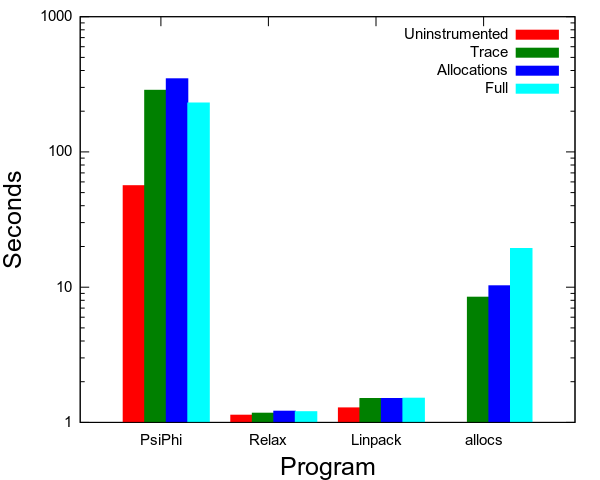
\includegraphics[width=\linewidth]{images/dbg/mtrace/performance}

  \caption{Performance of our evaluation programs under different
  instrumentation scenarios. Note logarithmic scale.  `Uninstrumented'
  is performance of the simulation without our interference. `Trace'
  interrupts for allocations; `mallocs' \emph{reports} allocations as
  well, which requires reading more data from the instrumented program.
  `Full' does allocation tracking, access detection, analysis, and
  visualization of the data.}

  \label{fig:performance}
\end{figure}

In practical terms, the performance scales with 1) the number of
allocations the program performs, and 2) the number of allocations that
are tracked and provide source locations for analysis.  Reducing the
number of allocations requires changing the programs of interest, which
is counter to our goal of a transparent solution.  However, avoiding
the tracking infrastructure for memory that the user is not interested
in is a plausible practical mechanism by which the user can influence
the performance of the instrumented system.

In many simulations, there is a large set of allocated memory that
is uninteresting from a visualization perspective.  Examples would
include data allocated internally to the C runtime or as a buffer for
I/O operations, in addition to simulation-allocated memory that simply
is not related to the underlying physics of interest.  To assist in
real-world usage, we provide a number of filters that ignore such
regions, much as Valgrind ignores known problems within e.g.
\textit{glibc}.  Furthermore, we provide a mechanism for the user to
mark memory regions as uninteresting.  This marking can be performed up
front, by
specifying a rule such as ``\textit{size $\geq$ 42}'', or in an
\textit{ad hoc} manner, by selecting a region explicitly.  Regions
ignored in this manner create no overhead, as observers for events
affecting them are removed as opposed to ignored.

% the tool has 0 overhead!
%% interrupting the program with ptrace is cheap
%% building the CFG is amortized over the accesses
%% symbolic execution is free due to the limited setting
%%%% in enzo, the average # of instructions in a basic block we hit is <X>
%% interrupting during accesses is not too expensive
%%%% we only interrupt the first access per function
%%%% only for memory we care about (i.e. not all accesses)
%%%% user can drop memory from the set of things we care about, improving perf
% reference hatcher again?

%\section{Overview}

%As in Figure~\ref{fig:teaser}, we seek to create a program that takes
%a program as well as a data model as input, and creates a set of
%visualizations.  These visualizations utilize a user-selected subset of
%the intermediate or output data evolved during the normal execution of
%the simulation program.  Visualizations are automatically updated as
%execution proceeds.

%\todo{have a screenshot of a user double-clicking the name of a
%variable and seeing a volume rendering of that data.}

%At its core level, our visual debugger will control the execution of
%the simulation via the \texttt{ptrace(2)} system call.  At important
%instants during simulation execution, the controlling process pauses
%the simulation process to inspect state and reverse-engineer the
%code from the instruction stream.  By successively eliminating
%possible interpretations of data, the controller can come to a unique
%understanding of these data and thereby create relevant visualizations.
%The controller knows when stale visualizations must be updated through
%updates to the underlying data.

%\subsection{Assumptions}
%\label{sec:assumptions}

%\todo{this gets very specific very quickly, we need more overview (or
%overview earlier) as to the vision for the whole thing}
%
%\begin{itemize}
%
%  \item visualizable data of interest are held in dynamic memory, and
%
%  \item arrays/data accessed in loops are contained in those loops
%  because the loop variable indexes the array, and
%
%  \item bounds on loop variables as found in loop headers imply bounds
%  on arrays accessed within the loop, and
%
%  \item the application does not use \texttt{goto}s from outside to
%  inside a loop in performance-critical code, and
%
%  \item a subset of optimizations related to code motion, notably loop
%  tiling, are not performed, and
%
%  \item debug information is available.
%
%  \todo{autovec doesn't happen?}
%
%\end{itemize}

%These assumptions are not onerous restrictions for the subset of
%programs used in simulation-based science.  As simulation data may be
%potentially large, it must be held in dynamic memory.  The `large'
%memory model popular in Fortran77 compilers violates this restriction,
%but this is being phased out by Fortran90+'s superior
%\texttt{allocatable} memory.

%\todo{better: ``we have found these assumptions to mostly be valid,
%one exception is e.g. fortran77's `large' memory model''. the idea is
%wording it so that fortran is just one example}

% Our loop bound assumptions are, at first glance, easier to violate.
% However, we note that we target a domain that is unusually focused on
% high-performance code.  If an array is accessed within a loop, but the
% index is not a function of the loop variable, then both the programmer
% as well as the compiler are likely to hoist this access outside of
% the loop.  Otherwise the access is redundant and an obstacle to the
% high-performance sought by simulation authors.

% The restriction on \texttt{goto} is a potential issue.
% High-performance code of interest may indeed utilize \texttt{goto}.
% However, we note that only a particular class of \texttt{goto} usage
% will violate our assumptions.  Furthermore, the construct has been in
% decline since Dijkstra's paper that argues the construct is harmful.
% \todo{other arguments why this isn't a big deal?}

% The optimization assumptions are particularly difficult, as these are
% dealt with on a case-by-case basis. Furthermore, each compiler will
% approach this problem differently.  However, \todo{[Someone] shows
% that loop tiling operations in C are extremely difficult to apply in
% practice [cite Someone here].}  Finally, considering our stated goal
% is minimizing the edit-compile-test cycle for simulation development,
% optimizations that defeat our analysis could simply be disabled during
% development.

%\todo{add a future work, maybe: tracking first and last access to an
%array so that i can detect issues with tiling, or the issue i'd have
%getting/using the wrong base address (the one of the allocation) when
%tiling/etc. hits us}

%\subsection{orig}

% Abstract interpretation is a promising approach to glean the properties
% we require for fitting memory to the given data model.  However,
% a straightforward interpretation approach is quickly stymied by
% computational cost.  Without bounds on the input, bounds on metadata
% can be wildly inaccurate, and we require exact sizing information for
% visualization.  Consider the relatively simple case of identifying the
% size of a dynamically-allocated array: the \texttt{malloc} argument is
% unlikely to be deterministic without the initial state of the program.
% Worse, even given the initial state, propagating this analysis is at
% least as expensive as executing the program.

% Consider the relatively simple case of identifying the
% size of a dynamically-allocated array: the \texttt{malloc} argument is
% unlikely to be deterministic without the initial state of the program.
% Worse, even given the initial state, propagating this analysis is at
% least as expensive as executing the program.
%
% Dynamic instrumentation is plagued with similar cost issues.  Software
% developers greatly value Valgrind\cite{Nethercote:2007:Valgrind} for
% its unwavering ability to identify memory errors, yet the software is
% rarely noted for its performance.
%
% The na\"ive application of both of these ideas is the primary cause
% of the computational explosion.  Our desire is to understand data
% structures, a task that is grossly more modest than whole program
% understanding.  Much code in a program has little to do with data
% structures.  A vastly smaller set of code is concerned with the
% manipulation of our data of interest: large 3D arrays.  By limiting
% our approach to only these regions, we can drastically cut the
% computational cost.

%\section{Large array identification}
%
%Any memory block in a simulation process' address space is a potential
%candidate
%for \textit{in situ} visualization.  However, only a small fraction
%of this memory is of practical interest.  Large amounts of memory are
%consumed by library code and the runtime stack, among other things.

%As per our assumptions, data of interest are heap-allocated.  Thus we
%expend effort identifying and tracking dynamically-allocated memory
%regions.

%\subsection{Tracking allocations}
%
%To identify memory regions of interest (i.e., visualizable data), we
%track all the allocations in a program.  When an allocation occurs,
%the simulation is temporarily paused.  We investigate the current
%state of the stack to identify the size as well as the memory address
%that was allocated, and then continue the execution of the simulation.
%Breakpoints implement this pause and continue cycle.

%We track allocations via breakpoints on both \texttt{malloc} and
%\texttt{free}.  Testing has shown that C++ and Fortran95 allocation
%routines boil down to these functions on all of GNU, Intel and LLVM
%implementations readily available to us.

%In practice, this produces a multitude of false positives: not all
%dynamic allocations are interesting sources for visual analysis.
%Almost all programs perform some level of string manipulations that
%directly or indirectly cause many allocations, for example.  We
%threshold our list by tracking only allocations above a particular
%size.
%\todo{Furthermore, by examining the debug information for the
%destination of the allocation, we can eliminate certain allocation
%classes (i.e. string allocations).}

%Processes that produce invalid memory operations may be exarcerbated
%by our modifications of the simulation's execution.  Handling such
%programs is beyond the goals of our work: conventional debugging
%techniques should be applied first.  Generally,
%Valgrind~\cite{Nethercote:2007:Valgrind}-clean operation is enough to
%guarantee our analysis is valid.

% \section{Symbolic and concrete execution}
%
% \todo{lorem ipsum dolor sit amet...}

%\section{Identifying loop bounds}

%Identifying the loop headers is an analysis on the program's control
%flow graph.  We compute only the control flow graph local to a function
%of interest due to the expense of the graph's construction.  Dominance
%information is computed via a textbook
%algorithm~\cite{Torczon:2007:Compiler}, but further analysis is needed
%to identify loop headers and a property we refer to as `depth'.  Depth
%is a count of the number of loops that a region of code is contained
%within.

%\subsection{Instruction parsing}

%The loop bound information is contained within the basic blocks that
%form loop headers and the memory of the simulation code.  However,
%identifying the data's source is nontrivial, due to the plethora of
%options that the compiler has for encoding a loop header.  While the
%options for the exact instruction sequence are numerous, we note that
%they are finite and all lead to an unambiguous conclusion concerning
%the data source.  For brevity, we detail the approach for a specific
%case and hint at the changes needed to support the full set of cases.

%Our example will use the instruction sequence from
%Listing~\ref{lst:header}.  This sequence of instructions copies two
%values from memory into registers, does a comparison between the two
%registers, and jumps to a new basic block based on the comparison.  The
%two values are the loop index and the loop bounds.  Of particular note
%is the source of data: one source is relative
%to the \texttt{rip} register, which is the instruction pointer in
%x86-64.  The second is relative to the \texttt{rbp} register, otherwise
%known as the frame pointer.

%\todo{this is essentially written in a `the way we want it to work,
%X, cannot work, so we do Y' style, but maybe we should flip it to be,
%`we do Y, which would be better as X but X is too expensive because
%Reason'}

%The most important instruction is the \texttt{CMP}.
%Unfortunately, a myopic view of this instruction leaves a
%nondeterministic interpretation of its arguments.  Either \texttt{rdx}
%or
%\texttt{rax} could be the bound we seek; worse, as registers are
%untyped, we have no ability to interpret the byte sequences within
%these registers.  Importantly, we must discern between signed and
%unsigned values, integer or floating point, and pointer versus
%primitive types.  We can obtain this required binary descriptor by
%correlating
%the \emph{source} of the data in the comparison instruction with the
%debug information available for that source.

%\begin{algorithm}
%  \caption{Symbolic interpretation algorithm for identifying data sources.}
%  \label{alg:sinterp}
%  \begin{algorithmic}[1]
%    \State register[*] := UNKNOWN
%    \State instruction := start of basic block
%    \Repeat
%      \If{instruction.Opcode = MOVE}
%        \State mov := (MovInstruction)instruction
%        \If{mov.source $\in$ register}
%          \State register[mov.target] := register[mov.source]
%        \ElsIf{mov.source is an address}
%          \State register[mov.target] := mov.source
%        \EndIf
%      \EndIf
%%      \If{instruction.Opcode = ADD}
%%        \State add := (AddInstruction)instruction
%%        \If{add.dest $\in$ register $\land$ register[add.dest] $\neq$ UNKNOWN}
%%          \State register[add.dest] += add.source
%%        \EndIf
%%      \EndIf
%      \State instruction := next(instruction)
%    \Until instruction.Opcode = CMP
%  \end{algorithmic}
%\end{algorithm}

%Algorithm~\ref{alg:sinterp} derives the data source information.  We
%create a symbolic representation of the architecture's register file.
%The
%source of data in each register is initialized to the \texttt{UNKNOWN}
%state.  Move instructions will initialize the symbolic register's value
%with the address of the data being loaded.  Instructions that do not
%move data simply copy the information from the previous instruction.
%We continue until we hit the comparison instruction of interest.  The
%output of the algorithm is a symbolic register file that can be used to
%query the source of data in a comparison instruction.

%Note that the algorithm relies on implicit state that is guaranteed
%externally.  For example, there cannot be more than a single compare
%within this instruction sequence, as this would create a different
%basic block and our analysis is local to a single block.  Furthermore,
%the basic block under interpretation must load the data of interest
%from memory as opposed to relying on its presence from a preceding
%basic
%block.\todo{Actually, this state/assumption is not guaranteed to be
%valid.  The compiler
%\emph{could} decide to keep the loop bound in a register the whole
%time, for example.  I've never seen this happen, which I attribute to
%two reasons: the compiler cannot prove that the loop bound does not
%change (imprecise alias analysis?), and register pressure on x86.}

%To discern the actual values, execution of the simulation is continued
%up until
%the \texttt{CMP} instruction.  The \texttt{ptrace(2)} system call is
%then used to pull the register values from the simulation, and the
%addresses from the symbolic register file are used to query the debug
%information for the simulation, allowing the register values to be
%interpreted.  Once a correct interpretation is possible, the larger of
%the two arguments is assumed to be the loop bound.

%\todo{The system is currently vulnerable to code that uses pointer
%comparisons instead of indices to bound access to a visualizable field.
%We know which registers hold pointers, though (due to
%Algorithm~\ref{alg:sinterp}), and presumably
%\emph{could} discern and then properly interpret this case.}

%Variations on the above theme cover alternative cases.  One example
%is the comparison instruction directly referencing memory, instead
%of pulling data into a register with a previous move instruction,
%obviating the need for the symbolic register file.  Another is the loop
%index counting from the bound down to 0.  Multiple iterations must be
%observed in this case, and the maximum value seen is taken.

%Astute readers will note that the implicit assumption that a data array
%accessed within a loop does not strictly implicate that the loop bound
%applies to that data array.  In a manner similar to identifying the
%source of operands in the compare instruction, one could verify that
%the loop indices are utilized when indexing the data of interest.  In
%practice, we have not found this to be necessary: if an array access
%is not dependent on the loop index, authors will move the access
%outside of the loop.  In some cases, the compiler may prove the index
%independence and hoist the access itself.
%
%\todo{what about autovectorization?}
%
%\subsection{Data access identification}
%%
%The creation and analysis of the control flow graph is on the order
%of tens of milliseconds for small test programs.  However, for `real
%world' programs this analysis scales poorly.  To make this process
%feasible, we aggressively localize the analysis.
%Algorithm~\ref{alg:sinterp} runs only within relevant loop header
%basic blocks.  Another method we use for localizing the analysis is by
%building only the local control flow graph in the areas where data are
%accessed.
%
%Modern data flow analysis is \todo{(is it really?)} capable of
%tracking data from allocation to its access and use.  However,
%the intractability of alias analysis is a significant barrier
%to application in this context.  An alternative option would be
%dynamic instrumentation a la Valgrind, however this would incur a
%prohibitive per-memory-access penalty.  Debug registers as used to
%implement watchpoints in debuggers are yet a third option, but popular
%architectures such as x86-64 have a limit of four such registers.
%
%The solution we utilize is based on an approach pioneered for
%distributed shared memory.  In these systems, data are presented as
%if the entirety of a large distributed array is local to a single
%node.  However, only the parts local to that process are mapped into
%the processes' address space.  Accessing remote regions produces a
%segmentation fault that is caught and used to identify the remote
%machine that houses the required data.  After the remote data have been
%copied locally, the instruction that produced the segmentation fault is
%restarted and normal operation is resumed.

%We utilize a similar scheme to identify data access locations.  When
%data are
%allocated, we silently and transparently replace the \texttt{malloc}
%function with calls to our custom implementation in
%Listing~\ref{lst:malloc}.  The purpose of this function is to
%write-protect the allocation of the field.  Execution is then
%resumed at native speed.  When the simulation reaches a point where
%the allocated memory is modified, execution will pause due to a
%segmentation fault.  The address of the instruction that caused the
%segmentation fault is the starting point for our analysis: we create
%and analyze the control flow graph only for the function that contains
%that instruction.  After analysis is complete, we unprotect the memory
%and resume execution at the previous instruction.  The protection is
%reinstated at the exit point from the current function.
%
%This approach has a number of advantages.  The primary motivation
%is its performance.  As the access privileges are checked via the
%hardware's memory management unit (MMU), it incurs no additional overhead
%during normal operation.  Replacing \texttt{malloc} with a more
%complicated allocation is negligible, as allocations are already
%expensive operations.  Write access incurs a context switch and two
%additional
%\texttt{mprotect} calls to disable and re-enable protection.
%\todo{or worse? what is the actual overhead?}  Unlike debug registers,
%per-page memory protection is not a limited resource.


\section{Related work}

\textit{In situ} visualization has a rich history in the visualization
community.  Recent frameworks include Damaris/Viz, the ParaView
Coprocessing library, and VisIt's `libsim'~\cite{Dorier:2013:Damaris,
Fabian:2011:Catalyst, Whitlock:2011:Libsim}. Dorier et
al.~\cite{Dorier:2013:Damaris} open
by noting the important factors for an \textit{in situ} visualization
tool. Among these factors are \textbf{low impact on code} and
\textbf{low impact on runtime}.  As our solution requires zero code
modifications, it has the lowest impact on the simulation code of any
\textit{in situ} visualization tool.  Performance is viable in
favorable conditions, and we hope to lower the overhead in the future.

Debugging high-performance computing applications is especially important as
parallelism increases and debugging becomes correspondingly more difficult.
\cite{Laguna:2011:Debugging} extend their earlier
work~\cite{Bronevetsky:2010:AutomaDeD} with a scalable method to
identify divergent parallel processes based on reduced control flow and
call stack information. Gao et al.~\cite{Gao:2007:DMTracker} watch
data movement patterns of a parallel application and use anomalies to
statistically infer a set of undesirable program activites.
\cite{Luecke:2003:MPICheck} instruments an MPI program to detect
invalid or inconsistent usage of the library.  All of these debugging
techniques are focused on identifying and eliminating the source of
programming-level errors, such as data corruption, deadlock, or
livelock.  In contrast, our \textit{ad hoc} visualization approach
would be more appropriate to identify algorithmic errors, such as
non-convergent error smoothing.

\cite{Rosenblum:2011:Authors} use program control flow graphs and a
custom-defined set of stylistic considerations to classify programs by
their authors given only the input binary.
\cite{Bernat:2012:BinEdit} define a number of `safe' control flow graph
transformations and an algebra for describing and deriving new ones.
Our code injection for page-aligned allocation is straightforward and
undeserving of such a robust formalism.

Our approach must identify and verify memory regions and related
variables that meet a set of invariants. McCloskey et
al.~\cite{McCloskey:2010:Infer} provided both a language and an
implementation to specify complex invariants suitable for our analyses.
\cite{Nguyen:2012:Invariants} use dynamic analysis to identify detailed
invariants that include array accesses.  Our approach utilizes
invariants that include reasoning at different levels, such as control
flow, in addition to invariants like those discovered therein.
\cite{Sharma:2013:DDEC} implement equivalence identification for
instruction-level loops.  Our code injection and access detection might
be seen as a lighter weight variant of their sandboxing technique.  The
techniques in~\cite{Sharma:2013:DDEC} present a potential vector
for inferring bounds from pointer-based loop guards, by deriving
equivalent index-based guards and relying on our existing analysis
infrastructure.

\section{Conclusion}

% we have made simulationa and visualization easy to couple
% hit primary goal
% demonstrated that (with certain assumptions) compilation is not lossy
% drawbacks:
%% we can only reason about block data (arrays) right now
%% no solution for distributed data
%%

We have elucidated a method and demonstrated a prototype that
eliminates the surface area between simulation code and visualization
tool.  The dynamic instrumentation-based method is robust across
different domains in high-performance computing.  The approach solves a
data understanding and metadata communication problem while remaining
flexible in the visualization choices, allowing \textit{ad hoc}
visualization methods or the ability to leverage the large body of work
performed in the visualization community.

The primary goal of minimizing the integration effort for \textit{in
situ} visualization has been met.  Simulation authors need only
apply our work to their binary to instantly gain a window into their
calculations.  This was possible by using the running process'
instructions as well as the program's debug information to recover the
structure and meaning of simulation software from the compiled binary.
The restrictions we impose, including restrictions on how
\texttt{goto}s are used, ensure this decompilation is robust without
posing onerous requirements on the simulation developer.

%We have elucidated a mechanism that eliminates the surface area between
%simulation software and visualization tool.  The mechanism can be
%applied to
%either simplify existing \textit{in situ} visualization tool couplings,
%or can be used to generate novel visualizations.  The level of
%simplification is large enough to completely eliminate manual efforts
%in coupling visualization and simulation software.  It works without
%introducing an additional layer of abstraction; instead, it utilizes
%the specification already provided.

The approach is not without drawbacks.  We have presently only
validated the idea for single kind of simulation data: $N$-dimensional
arrays.  While we believe extensions to other mesh types are possible,
we leave this to future work.  Simulation software is typically
parallelized, yet we operate on a process level; it remains to be
seen how one might combine data from multiple sources to create
visualizations of the distributed domain.

The work here demonstrates that the metadata needed to make sense of
data structures is present in the binary as well as the source code, if
one is willing to work to extract it.  It represents a promising step
along the way of automatic \textit{in situ} visualization that we hope
to see extended in the future.

\subsection{Future work}

Integer-based or pointer-based loop indices is an input to our model
that the user must specify, with ill-developed semantics for the
pointer case.  In the future, we hope to detect this case using
debug information to automatically choose between the two.  Pointer
comparisons as opposed to integer indices may pose issues due to the
ambiguous mapping from the addresses to indices accessed.  We plan to
assume a linear traversal of the data and compute the indices based on
the allocation's type as well as the starting and ending indices.

Our preliminary prototype is already eminently useful.  However, there
are still a number of cases where the inference fails.  We hope to
incorporate a feedback loop with the user so that they may create
visualizations for memory that has not been accessed recently, or
adjust the parameterization should it exhibit subtle errors.

While we have connected our analysis with visualization software in an
\textit{ad hoc} manner, our primary focus thus far was to evaluate
whether the analysis was complete enough to derive metadata needed for
visualization.  To make a tool useful to simulation developers, we will
connect our inference tool to an existing \textit{in situ}
visualization tool, such as VisIt~\cite{Childs:2012:VisIt} or
ParaView~\cite{Fabian:2011:Catalyst}.

% Withheld for double blind review.
%\section{Acknowledgements}
%
% The authors thank Alexander Schiewe, Chuck Hansen, Chris Johnson, Pat
% McCormick, and Matt Might for insightful discussions.
%
% This work was supported by ...
